
\section{Kondensator I}
\label{section:kondensator_1}
\begin{frame}%STARTCONTENT

\frametitle{Kapazität}
\begin{itemize}
  \item Wichtigste Eigenschaft des Kondensators: Ladung speichern
  \item $\rightarrow$ Kapazität
  \end{itemize}
$C = \dfrac{Q}{U}$

\begin{itemize}
  \item mit $Q$ als elektrische Ladung
  \item Einheit: $\frac{As}{V}$ bzw. Farad $F$
  \item Die Kapazität ist die elektrische Ladung pro Volt
  \end{itemize}

\end{frame}

\begin{frame}
\frametitle{Kapazität durch Bauart}
\begin{columns}
    \begin{column}{0.48\textwidth}
    \begin{itemize}
  \item Die Kapazität kann durch die Bauart erreicht werden
  \end{itemize}
$C = \dfrac{\varepsilon_0 \cdot \varepsilon_r \cdot A}{d}$

\begin{itemize}
  \item $\rightarrow$ Kapazität ist größer bei größerer Fläche, kleinem Abstand oder anderem Dielektrikum
  \end{itemize}

    \end{column}
   \begin{column}{0.48\textwidth}
       \begin{itemize}
  \item $\varepsilon_0 = 0,855 \cdot 10^{-11}\frac{As}{Vm}$: elektrische Feldkonstante
  \item $\varepsilon_r$: relative Dielektrizitätszahl, abhängig vom Dielektrikum (ohne Einheit)
  \item $A$: Fläche der Kondensatorplatten
  \item $d$: Abstand der Platten
  \end{itemize}

   \end{column}
\end{columns}

\end{frame}

\begin{frame}
\only<1>{
\begin{QQuestion}{EA101}{Welche Einheit wird üblicherweise für die Kapazität verwendet?}{Amperestunden (Ah)}
{Ohm ($\Omega$)}
{Farad (F)}
{Henry (H)}
\end{QQuestion}

}
\only<2>{
\begin{QQuestion}{EA101}{Welche Einheit wird üblicherweise für die Kapazität verwendet?}{Amperestunden (Ah)}
{Ohm ($\Omega$)}
{\textbf{\textcolor{DARCgreen}{Farad (F)}}}
{Henry (H)}
\end{QQuestion}

}
\end{frame}

\begin{frame}
\only<1>{
\begin{QQuestion}{EC205}{Von welcher der nachfolgenden Größen ist die Kapazität eines Plattenkondensators \underline{nicht} abhängig?}{Plattenabstand}
{Spannung}
{Plattenfläche}
{Dielektrikum}
\end{QQuestion}

}
\only<2>{
\begin{QQuestion}{EC205}{Von welcher der nachfolgenden Größen ist die Kapazität eines Plattenkondensators \underline{nicht} abhängig?}{Plattenabstand}
{\textbf{\textcolor{DARCgreen}{Spannung}}}
{Plattenfläche}
{Dielektrikum}
\end{QQuestion}

}
\end{frame}

\begin{frame}
\only<1>{
\begin{QQuestion}{EC203}{Wodurch verringert sich die Kapazität eines Plattenkondensators? Durch~...}{eine größere Dielektrizitätskonstante des Dielektrikums.}
{einen größeren Plattenabstand.}
{eine größere Spannung.}
{größere Plattenflächen.}
\end{QQuestion}

}
\only<2>{
\begin{QQuestion}{EC203}{Wodurch verringert sich die Kapazität eines Plattenkondensators? Durch~...}{eine größere Dielektrizitätskonstante des Dielektrikums.}
{\textbf{\textcolor{DARCgreen}{einen größeren Plattenabstand.}}}
{eine größere Spannung.}
{größere Plattenflächen.}
\end{QQuestion}

}
\end{frame}

\begin{frame}
\only<1>{
\begin{QQuestion}{EC204}{In welchem Fall sinkt die Kapazität eines Plattenkondensators?}{Bei Vergrößerung der Plattenoberfläche}
{Bei Erhöhung der angelegten Spannung}
{Bei Vergrößerung des Plattenabstandes}
{Bei Vergrößerung der Dielektrizitätszahl}
\end{QQuestion}

}
\only<2>{
\begin{QQuestion}{EC204}{In welchem Fall sinkt die Kapazität eines Plattenkondensators?}{Bei Vergrößerung der Plattenoberfläche}
{Bei Erhöhung der angelegten Spannung}
{\textbf{\textcolor{DARCgreen}{Bei Vergrößerung des Plattenabstandes}}}
{Bei Vergrößerung der Dielektrizitätszahl}
\end{QQuestion}

}
\end{frame}

\begin{frame}
\frametitle{Drehkondensator}
\begin{columns}
    \begin{column}{0.48\textwidth}
    \begin{itemize}
  \item Eine Platte ist feststehend, die andere Platte kann rotiert werden
  \item Nur dort, wo die Platten sich überlappen, wirkt der Kondensator
  \item Die Fläche wird durch Drehung verändert $\rightarrow$ Änderung der Kapazität
  \end{itemize}

    \end{column}
   \begin{column}{0.48\textwidth}
       
\begin{figure}
    \DARCimage{0.85\linewidth}{840include}
    \caption{\scriptsize Drehkondensator}
    \label{e_kondensator_drehkondensator}
\end{figure}


   \end{column}
\end{columns}

\end{frame}

\begin{frame}
\only<1>{
\begin{QQuestion}{EC206}{Wie nennt man ein Bauelement, bei dem sich Platten auf einer isolierten Achse befinden, die zwischen fest stehenden Platten rotiert werden können?}{Drehkondensator}
{Styroflexkondensator}
{Keramischer Kondensator}
{Rotorkondensator}
\end{QQuestion}

}
\only<2>{
\begin{QQuestion}{EC206}{Wie nennt man ein Bauelement, bei dem sich Platten auf einer isolierten Achse befinden, die zwischen fest stehenden Platten rotiert werden können?}{\textbf{\textcolor{DARCgreen}{Drehkondensator}}}
{Styroflexkondensator}
{Keramischer Kondensator}
{Rotorkondensator}
\end{QQuestion}

}
\end{frame}

\begin{frame}
\frametitle{Elektrolytkondensator}
\begin{columns}
    \begin{column}{0.48\textwidth}
    \begin{itemize}
  \item Spezielle Bauform
  \item Ermöglicht große Kapazität
  \item Nur für Gleichspannung
  \item Polarität muss beachtet werden
  \end{itemize}

    \end{column}
   \begin{column}{0.48\textwidth}
       
\begin{figure}
    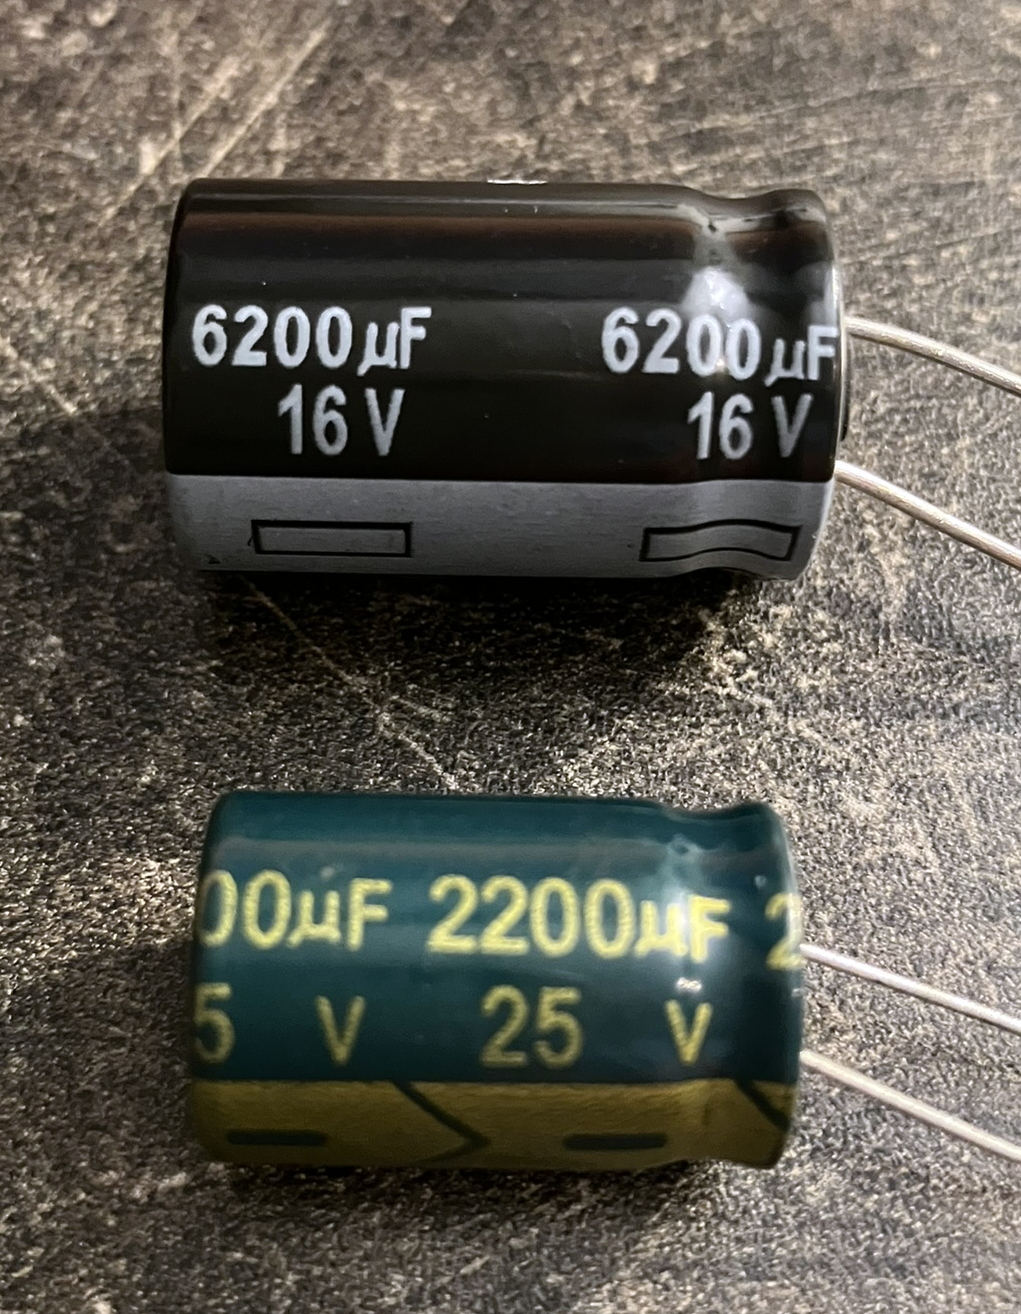
\includegraphics[width=0.85\textwidth]{foto/198}
    \caption{\scriptsize Elektrolytkondensatoren mit Markierung des Minus-Pols}
    \label{e_kondensator_elkos}
\end{figure}

   \end{column}
\end{columns}

\end{frame}

\begin{frame}
\only<1>{
\begin{QQuestion}{EC207}{Bei welcher der folgenden Bauformen von Kondensatoren muss beim Einbau auf die Polarität geachtet werden?}{Elektrolytkondensator}
{Keramikkondensator}
{Styroflexkondensator}
{Plattenkondensator}
\end{QQuestion}

}
\only<2>{
\begin{QQuestion}{EC207}{Bei welcher der folgenden Bauformen von Kondensatoren muss beim Einbau auf die Polarität geachtet werden?}{\textbf{\textcolor{DARCgreen}{Elektrolytkondensator}}}
{Keramikkondensator}
{Styroflexkondensator}
{Plattenkondensator}
\end{QQuestion}

}
\end{frame}

\begin{frame}
\frametitle{Ladekurve}
\begin{columns}
    \begin{column}{0.48\textwidth}
    \begin{itemize}
  \item Ein leerer Kondensator wird an Gleichspannung angeschlossen
  \item Die Spannung steigt steil an und flacht dann zur angelegten Spannung ab 
  \end{itemize}

    \end{column}
   \begin{column}{0.48\textwidth}
       
\begin{figure}
    \DARCimage{0.85\linewidth}{185include}
    \caption{\scriptsize Ladekurve eines Kondensators}
    \label{e_ladekurve_kondensator}
\end{figure}


   \end{column}
\end{columns}

\end{frame}

\begin{frame}
\only<1>{
\begin{question2x2}{EC201}{Welchen zeitlichen Verlauf hat die Spannung an einem entladenen Kondensator, wenn dieser über einen Widerstand an eine Gleichspannungsquelle angeschlossen wird?}{\DARCimage{1.0\linewidth}{188include}}
{\DARCimage{1.0\linewidth}{186include}}
{\DARCimage{1.0\linewidth}{185include}}
{\DARCimage{1.0\linewidth}{187include}}
\end{question2x2}

}
\only<2>{
\begin{question2x2}{EC201}{Welchen zeitlichen Verlauf hat die Spannung an einem entladenen Kondensator, wenn dieser über einen Widerstand an eine Gleichspannungsquelle angeschlossen wird?}{\DARCimage{1.0\linewidth}{188include}}
{\DARCimage{1.0\linewidth}{186include}}
{\textbf{\textcolor{DARCgreen}{\DARCimage{1.0\linewidth}{185include}}}}
{\DARCimage{1.0\linewidth}{187include}}
\end{question2x2}

}
\end{frame}

\begin{frame}
\frametitle{Kondensator im Wechselstrom}
\begin{itemize}
  \item Im Gleichstromkreis lädt der Kondensator sich auf, wirkt dann aber wie ein unendlich großer Widerstand
  \item Bei Wechselstrom wird der Kondensator ständig Auf- und Entladen
  \item Je höher die Frequenz, umso geringer ist der Wechselstromwiderstand des Kondensators
  \end{itemize}
\end{frame}

\begin{frame}
\only<1>{
\begin{QQuestion}{EC202}{Welches Verhalten zeigt der Wechselstromwiderstand eines idealen Kondensators mit zunehmender Frequenz?}{Er sinkt.}
{Er sinkt bis zu einem Minimum und steigt dann wieder.}
{Er steigt.}
{Er steigt bis zu einem Maximum und sinkt dann wieder.}
\end{QQuestion}

}
\only<2>{
\begin{QQuestion}{EC202}{Welches Verhalten zeigt der Wechselstromwiderstand eines idealen Kondensators mit zunehmender Frequenz?}{\textbf{\textcolor{DARCgreen}{Er sinkt.}}}
{Er sinkt bis zu einem Minimum und steigt dann wieder.}
{Er steigt.}
{Er steigt bis zu einem Maximum und sinkt dann wieder.}
\end{QQuestion}

}
\end{frame}%ENDCONTENT
